\section{Wall\-Iterator Class Reference}
\label{classWallIterator}\index{WallIterator@{WallIterator}}
{\tt \#include $<$walliterator.hpp$>$}

Inheritance diagram for Wall\-Iterator::\begin{figure}[H]
\begin{center}
\leavevmode
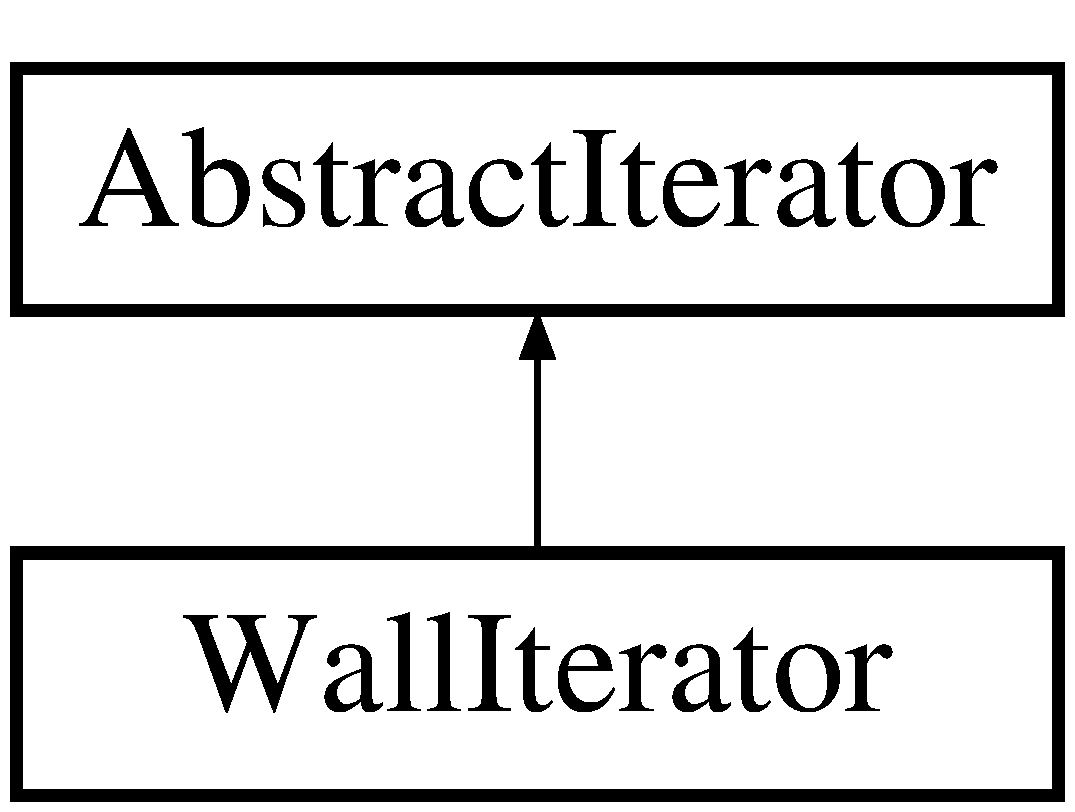
\includegraphics[height=2cm]{classWallIterator}
\end{center}
\end{figure}
\subsection*{Public Member Functions}
\begin{CompactItemize}
\item 
{\bf Wall\-Iterator} (int base\-X, int base\-Y, int width, int height)
\item 
bool {\bf operator!} ()
\item 
void {\bf operator++} (int)
\item 
int {\bf x} ()
\item 
int {\bf y} ()
\end{CompactItemize}
\subsection*{Protected Attributes}
\begin{CompactItemize}
\item 
int {\bf \_\-base\-X}
\item 
int {\bf \_\-base\-Y}
\item 
int {\bf \_\-x}
\item 
int {\bf \_\-y}
\item 
int {\bf \_\-w}
\item 
int {\bf \_\-h}
\item 
int {\bf \_\-phase}
\end{CompactItemize}


\subsection{Detailed Description}
Let x and y be coordinates so that 0$<$=x$<$width, 0$<$=y$<$height. Then if x==0 or x==(width-1) or y==0 or y==(height-1), it is a wall. Wall\-Iterator iterates these walls.



\subsection{Constructor \& Destructor Documentation}
\index{WallIterator@{Wall\-Iterator}!WallIterator@{WallIterator}}
\index{WallIterator@{WallIterator}!WallIterator@{Wall\-Iterator}}
\subsubsection{\setlength{\rightskip}{0pt plus 5cm}{\bf Wall\-Iterator} (int {\em base\-X}, int {\em base\-Y}, int {\em width}, int {\em height})}\label{classWallIterator_a0}




\subsection{Member Function Documentation}
\index{WallIterator@{Wall\-Iterator}!operator"!@{operator"!}}
\index{operator"!@{operator"!}!WallIterator@{Wall\-Iterator}}
\subsubsection{\setlength{\rightskip}{0pt plus 5cm}bool operator! ()\hspace{0.3cm}{\tt  [virtual]}}\label{classWallIterator_a1}




Implements {\bf Abstract\-Iterator} {\rm (p.\,\pageref{classAbstractIterator_a0})}.\index{WallIterator@{Wall\-Iterator}!operator++@{operator++}}
\index{operator++@{operator++}!WallIterator@{Wall\-Iterator}}
\subsubsection{\setlength{\rightskip}{0pt plus 5cm}void operator++ (int)\hspace{0.3cm}{\tt  [virtual]}}\label{classWallIterator_a2}




Implements {\bf Abstract\-Iterator} {\rm (p.\,\pageref{classAbstractIterator_a1})}.\index{WallIterator@{Wall\-Iterator}!x@{x}}
\index{x@{x}!WallIterator@{Wall\-Iterator}}
\subsubsection{\setlength{\rightskip}{0pt plus 5cm}int x ()}\label{classWallIterator_a3}


\index{WallIterator@{Wall\-Iterator}!y@{y}}
\index{y@{y}!WallIterator@{Wall\-Iterator}}
\subsubsection{\setlength{\rightskip}{0pt plus 5cm}int y ()}\label{classWallIterator_a4}




\subsection{Member Data Documentation}
\index{WallIterator@{Wall\-Iterator}!_baseX@{\_\-baseX}}
\index{_baseX@{\_\-baseX}!WallIterator@{Wall\-Iterator}}
\subsubsection{\setlength{\rightskip}{0pt plus 5cm}int {\bf \_\-base\-X}\hspace{0.3cm}{\tt  [protected]}}\label{classWallIterator_p0}


\index{WallIterator@{Wall\-Iterator}!_baseY@{\_\-baseY}}
\index{_baseY@{\_\-baseY}!WallIterator@{Wall\-Iterator}}
\subsubsection{\setlength{\rightskip}{0pt plus 5cm}int {\bf \_\-base\-Y}\hspace{0.3cm}{\tt  [protected]}}\label{classWallIterator_p1}


\index{WallIterator@{Wall\-Iterator}!_h@{\_\-h}}
\index{_h@{\_\-h}!WallIterator@{Wall\-Iterator}}
\subsubsection{\setlength{\rightskip}{0pt plus 5cm}int {\bf \_\-h}\hspace{0.3cm}{\tt  [protected]}}\label{classWallIterator_p5}


\index{WallIterator@{Wall\-Iterator}!_phase@{\_\-phase}}
\index{_phase@{\_\-phase}!WallIterator@{Wall\-Iterator}}
\subsubsection{\setlength{\rightskip}{0pt plus 5cm}int {\bf \_\-phase}\hspace{0.3cm}{\tt  [protected]}}\label{classWallIterator_p6}


\index{WallIterator@{Wall\-Iterator}!_w@{\_\-w}}
\index{_w@{\_\-w}!WallIterator@{Wall\-Iterator}}
\subsubsection{\setlength{\rightskip}{0pt plus 5cm}int {\bf \_\-w}\hspace{0.3cm}{\tt  [protected]}}\label{classWallIterator_p4}


\index{WallIterator@{Wall\-Iterator}!_x@{\_\-x}}
\index{_x@{\_\-x}!WallIterator@{Wall\-Iterator}}
\subsubsection{\setlength{\rightskip}{0pt plus 5cm}int {\bf \_\-x}\hspace{0.3cm}{\tt  [protected]}}\label{classWallIterator_p2}


\index{WallIterator@{Wall\-Iterator}!_y@{\_\-y}}
\index{_y@{\_\-y}!WallIterator@{Wall\-Iterator}}
\subsubsection{\setlength{\rightskip}{0pt plus 5cm}int {\bf \_\-y}\hspace{0.3cm}{\tt  [protected]}}\label{classWallIterator_p3}




The documentation for this class was generated from the following files:\begin{CompactItemize}
\item 
{\bf walliterator.hpp}\item 
{\bf walliterator.cpp}\end{CompactItemize}
